\subsection{Rolling Shutter Channel Model}
\subsubsection{Rolling Shutter Operation}

\begin{figure}[!t] %move forward
	\centering
	\begin{subfigure}[h]{0.3\textwidth}
		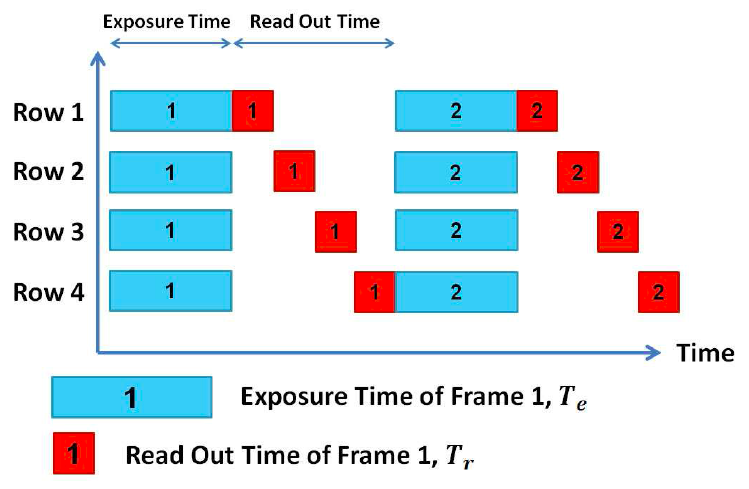
\includegraphics[width=\textwidth]{fig/global_shutter.png}
		\caption{Global Shutter Operation}
	\end{subfigure}
	~
	\begin{subfigure}[h]{0.15\textwidth}
		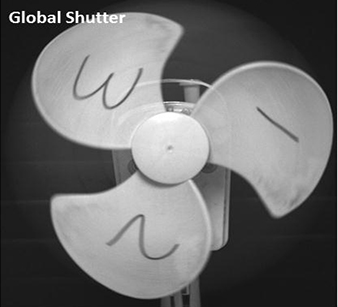
\includegraphics[width=\textwidth]{fig/fan_global}
		\caption{Global Shutter Example}
	\end{subfigure}
	\\
	\begin{subfigure}[h]{0.3\textwidth}
		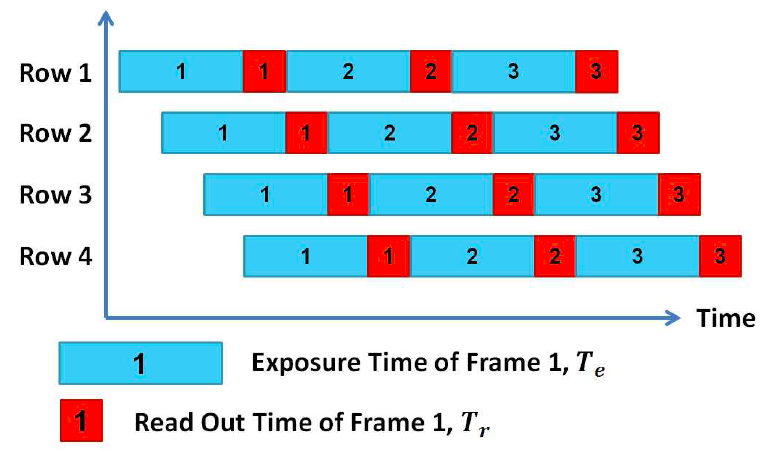
\includegraphics[width=\textwidth]{fig/rolling_shutter.png}
		\caption{Rolling Shutter Operation}
	\end{subfigure}
	~
	\begin{subfigure}[h]{0.15\textwidth}
		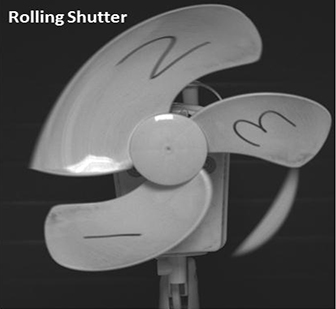
\includegraphics[width=\textwidth]{fig/fan_rolling}
		\caption{Rolling Shutter Example}
	\end{subfigure}
\caption{Shutter mechanisms}
\label{fig:compare_shutter}
\end{figure}

\autoref{fig:compare_shutter} compares global and rolling shutter operation \cite{imagesensor}. Global shutters, which are commonly implemented on CCD sensors, expose all pixels on the sensor simultaneously and gather incoming light over all pixels during the exposure time. 
Although some CMOS sensors use a global shutter, the majority found in the consumer market utilize a rolling shutter. 
One of the key properties of a rolling shutter camera sensor is its sequential read-out architecture. 
As in most CMOS sensors there is no per pixel storage to hold the accumulated charge during the exposure operation, the exposure period happens right before each read-out operation. 
The read-out architecture can process charge voltage signals one row at a time. 
Since the read-out durations of two rows cannot overlap, each of the exposure durations of a row of pixels is shifted by a fixed amount of read-out time (represented by $T_r$ in \autoref{fig:RollingShutter}), resulting in the so-called rolling shutter operation.
For each pixel, the incoming intensity modulated signal is integrated for a time period called exposure time (represented by $T_e$ in \autoref{fig:RollingShutter}). 

\begin{figure}[!t]
  \centering
  %\hspace{3em}
  % 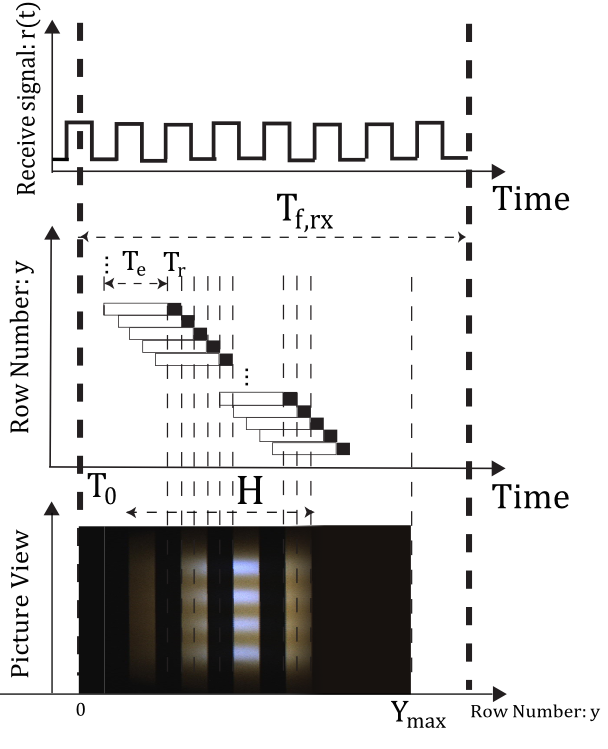
\includegraphics[scale=0.35]{fig/RollingShutter2}
  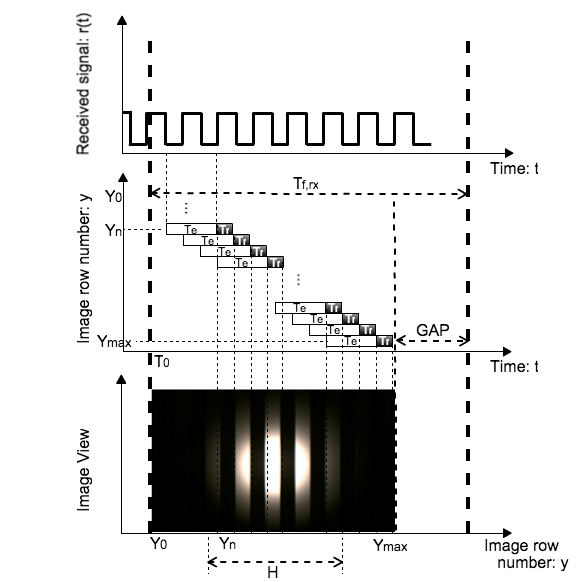
\includegraphics[scale=0.45]{pic/rollingshutter.png}
  \caption{The receiving operation of a rolling shutter camera sensor. Top: the original received signal; middle: the exposure and read-out processes; bottom: the resulted image. $T_{f,rx}$: receiving frame duration; $T_e$: exposure time; $T_r$: read-out time.}
  \label{fig:RollingShutter}
\end{figure}

\autoref{fig:RollingShutter} shows the receiving operation of a rolling shutter camera sensor to an intensity modulated signal.
Assume the original received signal in time is given by $r(t)$, which includes the signal from the transmitted light and other ambient interference. Considering the direct integration operation taking place during exposure and the rolling shutter operation, the intensity of a pixel in $y$-th row in the image, $I[y]$, which also represents the total amount of photons received by the pixel during exposure, is given by:

\begin{equation}
  I[y]=\int^{T_0+y T_r+T_e}_{T_0+y T_r} r(t) dt, \; 0 \leq y \leq Y_{\max},
  \label{eq:rollingshutter}
\end{equation}

where $T_r$ is the read-out time, $T_e$ is the exposure time, $T_0$ is a reference time point that corresponds to the start of the exposure time of the first row of pixels in the image, and $Y_{\max}$ is the number of rows of pixels in the image. Note that the transmitting light might not illuminate all rows in the image. In that case, the transmitted signal is only observed in $I[Y_{\operatorname{top}} \leq y \leq Y_{\operatorname{top}}+H]$, where $H$ represents the height of the image area illuminated by the transmitting light. 

The direct integration operation can be considered as a low-pass filter (or a moving average filter), and thus $I[y], 0 \leq y \leq Y_{\max}$ is a filtered version of the original received signal $r(t)$. The filter distorts high frequency components in the received signal, especially the ones with a frequency higher than $1/T_e$. 


\subsubsection{Time Gap in the Frame Duration}
Utilizing \autoref{eq:rollingshutter}, if the transmitting light occupies all rows of pixels in the image, the end of exposure of the last row in this image frame is $T_0 + Y_{\max} T_r + T_e$, while the start of exposure of the first row in the next image frame is $T_0 + T_{f,rx}$. The \textbf{time gap} between these two events is $T_{f,rx} - Y_{\max} T_r - T_e$, when $T_e$ is small, is significant for most cameras. 
This is the amount of time during which the camera is not performing any exposure operation, i.e., not receiving the transmitted signal. Signal transmitted during this time period is lost.  

\autoref{tab:readout} summarizes both the values of this time gap (without subtracting the exposure time $T_e$) and the percentage of time contributed by this time gap compared to a frame duration. Note that for some cameras, this could be up to half of the receiving frame duration. In addition, in the case that the transmitting light does not illuminate all rows in the image, this time gap could further increase. 

\subsubsection{Channel Characteristics}
In summary, the single-LED-to-rolling-shutter-camera channel exhibits two major characteristics:
\begin{enumerate}
  \item The signal that can be obtained from the image is a low-pass filtered version of the original received signal in time. The filter create distortions in high frequency components.
  \item The receiving process is not continuous. This can be considered as a form of channel fading; when it takes place, the channel loss is infinite. The ratio of signal lost is determined by a constant time gap that depends on camera parameters, and the size of the image area illuminated by the transmitting light. A smaller image area corresponds to a higher ratio of signal lost.
\end{enumerate}

